\chapter{基于前缀承载的水印算法}

\section{问题描述}

推理期文本水印的目标是在不显著破坏生成质量的前提下，使模型输出文本携带可被检测端识别的统计信号。然而，在真实传播环境中，生成文本往往会经历复制、改写、轻度润色以及字符级或 token 级编辑等后处理过程。这类编辑攻击不仅会改变文本的表面形式，还可能进一步引发分词结果变化，从而破坏检测端对生成端伪随机结构的复现，并削弱水印统计量的累积效果。Kirchenbauer 等\cite{kirchenbauer2024reliability}系统分析了人工改写、模型释义以及混合文本对水印可靠性的影响。Rastogi 等\cite{rastogi2024revisiting}进一步表明，黑盒场景下的释义攻击也可能显著削弱检出能力。进一步地，字符级扰动会额外引发分词边界变化。Zhang 等\cite{zhang2025character}指出，这类微扰容易通过分词级联效应放大检测退化；Liang 等\cite{liang2024waterpark}的综合评测也表明，高度依赖分词一致性的检测统计在此类攻击下更容易失效。因此，如何提高水印方法在分词扰动条件下的检测稳定性，是推理期文本水印在实际应用中面临的关键问题。

现有推理期水印方法通常在生成过程中依据密钥与上下文构造伪随机分区，并在此基础上对候选分布施加轻微偏置，使带水印文本在长文本范围内呈现可检验的统计差异，其中 KGW\cite{kirchenbauer2023watermark} 是这一范式的代表。此后，Unbiased Watermark\cite{hu2023unbiased}从无偏嵌入角度改进了这一框架，DiPmark\cite{wu2023dipmark}则进一步强调分布保持、可检测性与鲁棒性的兼顾。这类方法的有效性依赖两个基本前提：其一，水印信号所绑定的承载对象在生成端与检测端之间能够保持一致；其二，检测端能够依据相同的上下文重建与生成端一致的伪随机分区。然而，在分词扰动存在时，这两个前提都可能受到破坏。一方面，若水印信号直接依赖具体 token 身份，则编辑引起的分词变化会导致原有 token 对应关系发生漂移，使承载对象本身失稳；另一方面，若伪随机分区直接依赖精确的 token 上下文，则局部编辑还会进一步改变分区输入，使检测端难以稳定复现生成端使用的分区结构，从而削弱检测统计量。

针对上述问题，本文关注的核心问题是：在分词扰动条件下，如何构造一种对分词变化更不敏感的推理期文本水印方法，使水印信号在文本经历合理编辑后仍能够保持较好的可检测性。围绕这一目标，本文提出基于前缀承载的水印算法。该方法一方面将水印承载对象从易受分词影响的具体 token 身份提升到更稳定的前缀类别，以降低承载对象随分词边界变化而发生漂移的风险；另一方面，引入指纹驱动的伪随机分区机制，降低分区输入对局部上下文细微变化的敏感性，从而提高生成端与检测端在编辑扰动下构造一致统计结构的可能性。在此基础上，本文进一步设计相应的嵌入与检测流程，以提升水印在分词扰动条件下的鲁棒性。

\section{算法设计}

\subsection{整体框架}

为提高文本水印在分词扰动条件下的鲁棒性，本文从水印承载对象与伪随机分区结构两个层面进行联合设计。现有推理期文本水印通常在生成阶段依据密钥与上下文构造绿色集合，并对绿色集合中的候选施加轻微偏置，使水印信号在长文本中累积为可检验的统计差异，KGW 是其中的经典代表\cite{kirchenbauer2023watermark}。在此基础上，Unbiased Watermark 从无偏嵌入角度扩展了这一设计路线\cite{hu2023unbiased}，DiPmark 则进一步从分布保持角度推进了这一路线\cite{wu2023dipmark}。然而，当文本在传播过程中经历轻度编辑后，分词结果和局部上下文都可能发生变化。若水印信号直接依赖具体 token 身份，分词变化就会导致承载对象漂移；若绿色集合的构造直接依赖精确上下文，检测端又难以稳定复现生成端使用的伪随机分区结构。针对这两个问题，本文提出基于前缀承载的水印算法，将水印承载从具体 token 身份提升到更稳定的前缀类别，并引入局部上下文指纹驱动的伪随机函数（Pseudo-Random Function, PRF）分区机制，以降低分区输入对局部编辑的敏感性。

\begin{figure}[htbp]
    \centering
    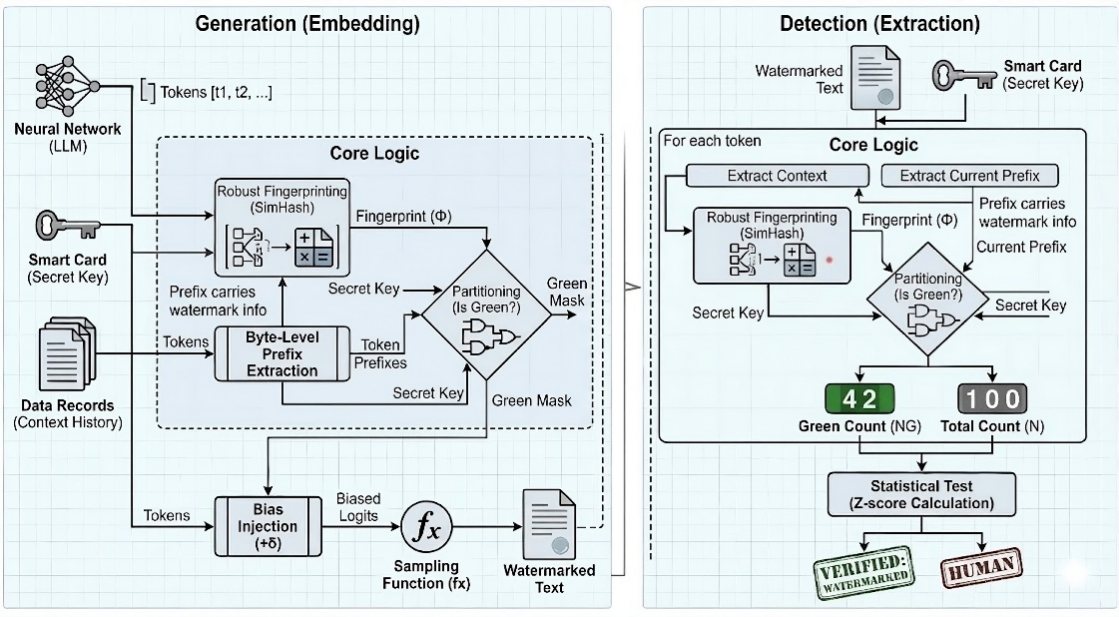
\includegraphics[width=0.95\linewidth]{figures/watermark_framework.png}
    \caption{基于前缀承载的水印算法整体框架}
    \label{fig:watermark_framework}
\end{figure}

如图~\ref{fig:watermark_framework} 所示，本文方法由生成端与检测端两部分构成。在生成端，给定当前位置之前的 token 前缀 $x_{<t}$，语言模型在词表 $V$ 上输出下一步候选分布
\begin{equation}
p_t(v)=p(v\mid x_{<t}), \quad v\in V,
\label{eq:wm_next_token_dist}
\end{equation}
其中，$p_t(v)$ 表示第 $t$ 步在上下文 $x_{<t}$ 下生成候选 token $v$ 的条件概率，$V$ 表示模型词表。随后，算法对每个候选 token 提取其对应的前缀类别，并从当前可见文本的局部上下文中构造稳定指纹。记候选 $v$ 的前缀类别为 $u_n(v)$，其中下标 $n$ 表示前缀长度；记第 $t$ 步由局部上下文得到的指纹为 $h_t$。在共享密钥 $k$ 的控制下，算法根据 $\bigl(u_n(v), h_t\bigr)$ 为每个候选确定其在当前步是否属于绿色集合 $G_t$，并在此基础上对绿色集合中的候选施加轻微偏置，再从偏置后的分布中完成采样，从而得到带水印文本。

在检测端，给定待检测文本后，算法按照与生成端一致的规则逐位置重建前缀类别与局部上下文指纹。具体而言，检测端首先从待检测文本中提取当前位置之前的可见上下文，并计算相应的指纹 $h_t$；随后，对当前位置 token 对应的前缀类别 $u_n(v)$ 进行判定，并利用相同密钥 $k$ 和相同的 PRF 复现当前步的绿色集合 $G_t$。在此基础上，检测端统计整段文本中的绿色命中次数与总计数，并进一步构造标准化统计量进行检验，从而判断该文本是否更可能来自带水印的生成过程。

上述整体框架包含三个关键组成部分。首先，前缀承载与类别标识用于定义更稳定的水印载体，从而降低分词边界变化对承载对象的直接破坏；其次，指纹驱动的 PRF 分区用于构造对局部编辑更不敏感的绿色集合，以提高生成端与检测端之间分区结构的一致性；最后，水印嵌入与检测在前两者基础上完成统计信号的注入与判别。三者共同作用，使得本文方法在文本经历合理编辑后，仍能够尽量保持可检测性。下面将分别介绍前缀承载与类别标识、指纹驱动的伪随机分区，以及水印嵌入与检测三个部分的具体设计。

\subsection{前缀承载与类别标识}

现有基于伪随机分区的推理期文本水印，通常以具体 token 身份作为水印承载对象，典型代表是 KGW\cite{kirchenbauer2023watermark}。后续如 Unbiased Watermark\cite{hu2023unbiased} 与 DiPmark\cite{wu2023dipmark} 也基本沿用了这一 token 级承载思路。更具体地说，在生成阶段，算法先依据密钥与当前上下文将候选 token 划分为绿色集合与非绿色集合，再通过提高绿色集合中候选的采样概率，使带水印文本在长文本范围内呈现出可检验的统计偏移。在这种机制下，水印信号的承载与累积依赖于当前位置实际输出的 token 是否被划入绿色集合。因此，传统方法隐含地要求：生成端与检测端在同一位置上看到的是相同的 token 身份，并且能够围绕该 token 身份复现一致的分区结果。

然而，在分词扰动存在时，这一承载方式会变得不稳定。少量字符级编辑虽然往往不会显著改变文本整体语义，但可能改变局部的分词边界，使原本对应于某一位置的 token 被替换、拆分或合并。Zhang 等指出，这类字符级微扰会通过分词级联效应放大检测退化\cite{zhang2025character}。Liang 等的综合评测也表明，高度依赖分词一致性的检测统计在此类攻击下更容易失效\cite{liang2024waterpark}。因此，即使可见文本变化有限，依赖具体 token 身份的水印承载对象也可能发生漂移，检测端据此重建的绿色命中序列随之失稳，从而削弱统计检验的有效性。因此，若希望提高水印在分词扰动条件下的鲁棒性，首先需要将承载对象从易受分词结果影响的具体 token 身份，转移到更稳定的表示层面。

基于这一考虑，本文不再直接以完整 token 身份作为承载对象，而是采用短前缀类别进行承载。具体而言，对于每个候选 token，算法不直接使用其完整身份参与后续分区与判定，而是仅提取其字节表示的前若干字节，并将具有相同短前缀的候选归入同一类别。这样做的好处在于，短前缀比完整 token 身份更粗粒度，因此对分词边界变化也更不敏感。换言之，即使轻量编辑导致 token 身份发生变化，新 token 在许多情况下仍可能与原 token 保持相同或相近的短前缀类别，从而降低水印承载对象发生漂移的概率。

需要进一步指出的是，前缀长度不能简单固定。若前缀过短，虽然类别更稳定，却会将大量候选压缩到少数类别中，使原始候选分布中的可用不确定性明显减少，进而削弱水印信号的承载空间；若前缀过长，则类别表示会重新接近具体 token 身份，前缀承载的鲁棒性优势也会随之减弱。因此，前缀承载的关键不在于是否采用前缀，而在于如何为当前步选择合适的前缀长度，使其在稳定性与可用信息量之间取得平衡。

为此，本文采用自适应前缀承载策略。设第 $t$ 步在上下文 $x_{<t}$ 下，语言模型在词表 $V$ 上给出的候选分布为
\begin{equation}
p_t(v)=p(v\mid x_{<t}), \qquad v\in V,
\label{eq:prefix_pt}
\end{equation}
其中，$p_t(v)$ 表示第 $t$ 步生成候选 token $v$ 的条件概率。对于任意前缀长度 $n$，都可以将候选 token 按其前 $n$ 个字节前缀聚合为类别分布。本文不直接固定某个 $n$，而是考察该聚合后仍保留了多少原始分布中的可用不确定性。为此，定义第 $t$ 步在前缀长度 $n$ 下的信息保留率为
\begin{equation}
\rho_t(n)=\frac{H_{\mathrm{pref}}(t,n)}{H_{\mathrm{full}}(t)},
\label{eq:prefix_rho}
\end{equation}
其中，$H_{\mathrm{full}}(t)$ 表示第 $t$ 步原始候选分布的熵，$H_{\mathrm{pref}}(t,n)$ 表示在前缀长度 $n$ 下的类别分布熵。$\rho_t(n)$ 越接近 $1$，说明当前前缀长度下仍保留了更多原始候选分布中的可用信息量。

在此基础上，本文引入信息保留阈值 $\eta$，并在每一步自适应地选择满足保留率要求的最短前缀长度。实验中取 $\eta=0.8$，即要求当前步至少保留约 $80\%$ 的可用不确定性。相应地，第 $t$ 步采用的前缀长度定义为
\begin{equation}
n_t=\min\{\, n \mid \rho_t(n)\ge \eta \,\}, \qquad \eta=0.8.
\label{eq:adaptive_prefix_length}
\end{equation}
该规则的含义是：在保证当前步仍有足够信息量可用于承载水印信号的前提下，尽量采用更短的前缀来提高对分词扰动的鲁棒性。因此，本文并不追求用更长前缀去逼近原始 token 身份，而是为当前步选择满足信息承载要求的最短前缀粒度。

\begin{figure}[htbp]
    \centering
    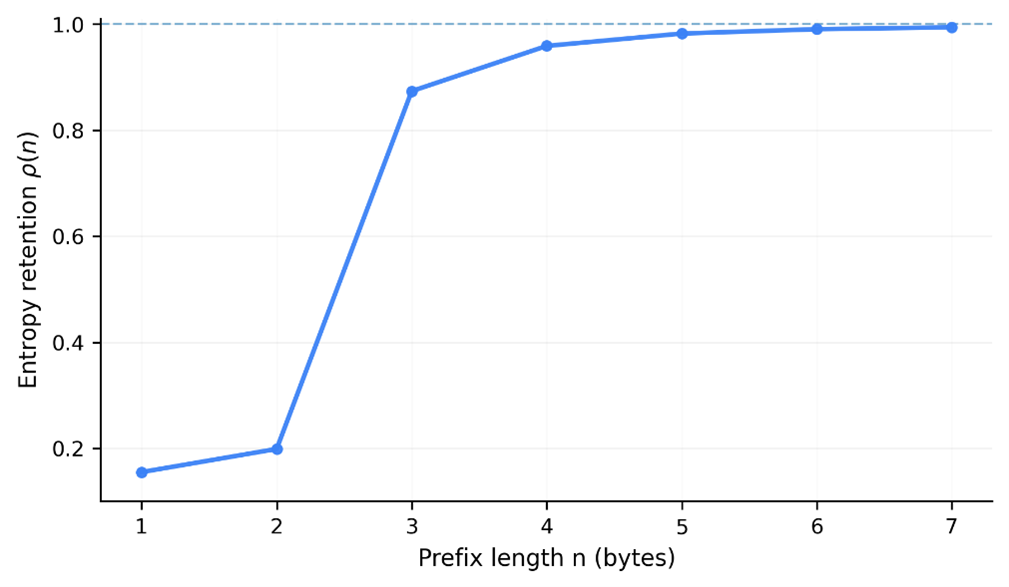
\includegraphics[width=0.78\linewidth]{figures/prefix_entropy_retention.png}
    \caption{不同前缀长度下的信息保留率示意图}
    \label{fig:prefix_entropy_retention}
\end{figure}

图~\ref{fig:prefix_entropy_retention} 给出了信息保留率随前缀长度变化的典型趋势。可以看到，当前缀长度较小时，类别聚合会明显压缩原始候选分布中的可用不确定性，因此信息保留率较低；随着前缀长度增加，保留率迅速上升并逐渐趋于饱和。这说明过短前缀虽然更稳定，但会损失过多可用信息，而继续增大前缀长度的收益又会逐步减弱。本文正是利用这一趋势，在每一步按照式~\eqref{eq:adaptive_prefix_length} 自适应选择当前承载粒度，而不是预先固定一个全局常数。

在当前步前缀长度 $n_t$ 确定之后，本文将每个候选 token $v$ 映射为对应的前缀类别，并以该类别作为后续伪随机分区与绿色集合判定的基本对象。记该类别标识为
\begin{equation}
u_t(v)=\mathrm{PrefixClass}(v;n_t),
\label{eq:prefix_class}
\end{equation}
其中，$u_t(v)$ 表示 token $v$ 在当前步自适应前缀长度 $n_t$ 下对应的前缀类别标识。后续算法不再直接依据原始 token 身份进行绿色判定，而是基于类别标识 $u_t(v)$ 进行伪随机分区与水印嵌入。这样一来，水印承载对象在分词扰动下更加稳定，同时又保留了足够的可用信息量，为下一节指纹驱动的伪随机分区提供了更稳健的基础对象。

\subsection{指纹驱动的伪随机分区}

上一节已经将水印承载对象由具体 token 身份转移为更稳定的前缀类别，从而降低了承载对象随分词边界变化而发生漂移的风险。然而，仅仅改变承载对象还不够。若绿色集合的构造仍然直接依赖精确的 token 上下文，则文本在传播过程中经历轻量编辑后，局部上下文的细微变化仍可能导致检测端难以稳定复现生成端使用的分区结构，进而削弱水印统计量。因此，在确定了承载对象之后，还需要进一步设计一种对局部编辑更不敏感、同时在生成端与检测端都可复现的伪随机分区机制。

基于这一考虑，本文采用指纹驱动的伪随机分区方法。其基本思想是，不再直接使用精确 token 上下文作为分区输入，而是先从当前位置之前的可见文本中提取一个固定长度的局部上下文指纹，再将当前候选的前缀类别通过密钥控制的伪随机函数（Pseudo-Random Function, PRF）映射为同维度的二进制类别向量，最后依据二者之间的汉明距离完成绿色集合判定。这样一来，分区机制不再直接依赖具体 token 身份和精确分词边界，而是建立在较为稳定的前缀类别与局部上下文指纹之上，从而提高分区结构在分词扰动下的可重建性。

\begin{figure}[htbp]
    \centering
    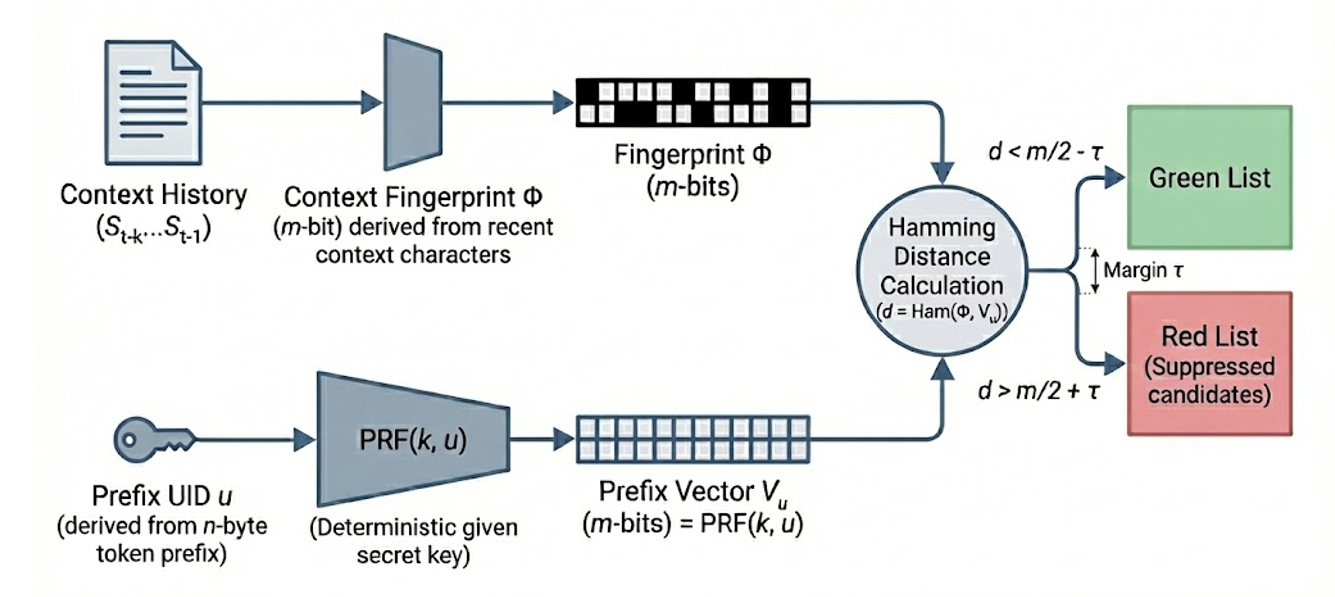
\includegraphics[width=0.90\linewidth]{figures/prf_partition.png}
    \caption{指纹驱动的伪随机分区示意图}
    \label{fig:prf_partition}
\end{figure}

如图~\ref{fig:prf_partition} 所示，图中所示的Prefix UID、Fingerprint和Prefix Vector分别对应本文的前缀类别标识、局部上下文指纹和类别向量。在第 $t$ 步，本文首先从当前位置之前的可见文本中截取最近的一段局部上下文，并将其映射为一个 $m$ 位二进制指纹，记为
\begin{equation}
h_t=\mathrm{FingerPrint}(s_{<t}) \in \{0,1\}^m,
\label{eq:context_fingerprint}
\end{equation}
其中，$s_{<t}$ 表示当前位置之前的可见文本前缀，$m$ 表示指纹维度。本文实现中采用基于 SimHash 的方式生成该局部上下文指纹，其目的在于将相近的局部上下文映射为相对稳定的二进制表示，从而减弱轻量编辑对分区输入的直接影响\cite{charikar2002similarity}。

另一方面，对当前候选 token $v$，上一节已经定义了其前缀类别标识 $u_t(v)$。本文利用共享密钥 $k$ 和伪随机函数将该类别映射为同样维度的二进制类别向量：
\begin{equation}
r_t(v)=\mathrm{PRF}_k\!\bigl(u_t(v)\bigr)\in \{0,1\}^m,
\label{eq:prefix_vector}
\end{equation}
其中，$\mathrm{PRF}_k(\cdot)$ 表示由密钥 $k$ 控制的伪随机函数，$r_t(v)$ 表示候选 $v$ 在当前步对应的类别向量。由于该映射仅依赖密钥和前缀类别，因此对于生成端与检测端而言都是确定且可复现的。

在得到局部上下文指纹 $h_t$ 与类别向量 $r_t(v)$ 之后，本文通过二者之间的汉明距离来完成当前候选的颜色判定。记
\begin{equation}
d_t(v)=\mathrm{Ham}\!\left(h_t, r_t(v)\right),
\label{eq:hamming_distance}
\end{equation}
其中，$\mathrm{Ham}(\cdot,\cdot)$ 表示汉明距离，$d_t(v)$ 表示当前上下文指纹与候选类别向量之间的距离。直观地看，当 $d_t(v)$ 较小时，说明当前候选类别与当前位置上下文在伪随机空间中更接近，可将其划入绿色集合；当 $d_t(v)$ 较大时，则将其划入非绿色集合。为增强判定稳定性，本文引入边界带宽参数 $\tau$，并按如下规则确定当前步的绿色集合：
\begin{equation}
G_t=\left\{\, v\in V \;\middle|\; d_t(v)<\frac{m}{2}-\tau \right\},
\label{eq:green_set}
\end{equation}
其中，$V$ 表示词表，$G_t$ 表示第 $t$ 步的绿色集合，$\tau$ 用于控制绿色判定与边界区域之间的间隔。对于距离落在边界带宽附近的候选，本文采用固定且可复现的判定规则，以避免轻微扰动引起频繁的颜色翻转。

上述分区方式的关键在于，绿色集合不再直接由精确 token 上下文决定，而是由局部上下文指纹 $h_t$ 与前缀类别 $u_t(v)$ 共同决定。由于前缀类别相比完整 token 身份更稳定，而上下文指纹相比精确上下文匹配也更能容忍局部细微变化，因此在文本经历轻量编辑后，检测端仍更有可能复现与生成端一致的分区结构。换言之，本文并没有改变 PRF 分区这一基本框架，而是通过更稳定的分区输入，降低了分区机制对分词边界和精确位置对齐的敏感性。基于该分区结果，下一节将进一步说明生成阶段如何注入水印偏置，以及检测阶段如何进行统计判别。

\subsection{水印嵌入与检测}

在前两节中，本文已经给出了当前步前缀类别 $u_t(v)$ 的构造方式，以及由局部上下文指纹 $h_t$ 驱动的绿色集合 $G_t$ 的判定规则。本节在此基础上说明生成端如何在绿色集合上注入水印偏置，以及检测端如何依据相同的规则重建绿色集合并完成统计判别。需要说明的是，本节中的水印检测并不是恢复某一显式消息，而是检验待检测文本是否呈现出带水印生成过程所诱导的系统性统计偏移。

在生成阶段，第 $t$ 步给定当前位置之前的 token 前缀 $x_{<t}$，语言模型输出词表 $V$ 上的原始 logits，记第 $v$ 个候选的 logit 为 $z_t(v)$。由此可得第 $t$ 步的原始条件分布
\begin{equation}
p_t(v)=\frac{\exp(z_t(v))}{\sum_{v' \in V}\exp(z_t(v'))}, \qquad v\in V,
\label{eq:wm_raw_dist}
\end{equation}
其中，$p_t(v)$ 表示在上下文 $x_{<t}$ 下生成候选 token $v$ 的原始条件概率。随后，算法根据前两节定义的前缀类别 $u_t(v)$、局部上下文指纹 $h_t$ 以及伪随机分区规则，构造当前步的绿色集合 $G_t \subseteq V$。在得到 $G_t$ 后，算法对其中候选施加偏置强度 $\delta>0$，并将偏置后的 logits 定义为
\begin{equation}
\widetilde{z}_t(v)=z_t(v)+\delta \cdot \mathbf{1}[v\in G_t],
\label{eq:wm_biased_logits}
\end{equation}
其中，$\mathbf{1}[\cdot]$ 为指示函数：当候选 $v$ 属于绿色集合 $G_t$ 时取值为 $1$，否则取值为 $0$。由偏置后的 logits 诱导的条件分布为
\begin{equation}
\widetilde{p}_t(v)=\frac{\exp(\widetilde{z}_t(v))}{\sum_{v' \in V}\exp(\widetilde{z}_t(v'))}, \qquad v\in V.
\label{eq:wm_biased_dist}
\end{equation}
最后，输出 token $y_t$ 由分布 $\widetilde{p}_t(v)$ 采样得到，并被追加到前缀中进入下一步生成。上述过程表明，水印偏置并不直接绑定于完整 token 身份，而是通过候选的前缀类别及其在当前绿色集合中的归属关系作用于候选分布。

在检测阶段，给定待检测文本后，算法沿序列逐位置遍历，并在每个位置重建与生成阶段一致的判定结构。设待检测文本在第 $t$ 步对应的 token 为 $y_t$。检测端首先根据当前位置之前的可见文本前缀恢复局部上下文指纹 $h_t$，再依据与生成阶段相同的规则计算该位置的前缀类别 $u_t(y_t)$，并在共享密钥 $k$ 下复现当前步的绿色集合 $G_t$。在此基础上，定义第 $t$ 步的绿色命中指示变量为
\begin{equation}
I_t=\mathbf{1}[y_t \in G_t],
\label{eq:wm_hit_indicator}
\end{equation}
其中，$I_t=1$ 表示当前位置 token 命中绿色集合，$I_t=0$ 表示未命中。为避免提示词区域或不参与判别的位置对统计结果造成干扰，本文使用位置集合 $\mathcal{T}$ 表示参与检验的有效位置集合。于是，在整段文本上的绿色命中数与总统计位置数分别定义为
\begin{equation}
N_G=\sum_{t\in \mathcal{T}} I_t,
\qquad
N=|\mathcal{T}|,
\label{eq:wm_ng_n}
\end{equation}
其中，$N_G$ 表示绿色命中次数，$N$ 表示参与统计的位置总数。

在无水印假设下，若绿色集合在统计上保持近似恒定的绿色比例 $\gamma$，则绿色命中数的期望约为 $\gamma N$。这里，$\gamma$ 表示无水印条件下任一位置命中绿色集合的基准概率，它由分区机制本身决定，并可通过理论分析或无水印样本估计得到。在此基础上，本文采用标准化统计量
\begin{equation}
z=\frac{N_G-\gamma N}{\sqrt{N\gamma(1-\gamma)}},
\label{eq:wm_zscore}
\end{equation}
其中，$z$ 表示绿色命中统计相对于无水印基准的偏离程度。当带水印生成过程持续提高绿色候选的采样概率时，$N_G$ 将相对无水印情形出现系统性偏大，从而使统计量 $z$ 上升。给定目标误报率（false positive rate, FPR）后，可确定相应的检测阈值 $z_{\mathrm{thr}}$。最终判决规则为
\begin{equation}
z>z_{\mathrm{thr}}
\;\Rightarrow\;
\text{判为带水印文本},
\qquad
z\le z_{\mathrm{thr}}
\;\Rightarrow\;
\text{判为无水印文本}.
\label{eq:wm_decision_rule}
\end{equation}

综上，本文的水印嵌入与检测流程建立在前缀类别和指纹驱动分区之上。生成端依据式~\eqref{eq:wm_biased_logits} 和式~\eqref{eq:wm_biased_dist} 在绿色集合上注入偏置，使绿色命中在长文本中形成可累积的统计偏移。检测端则沿用 Kirchenbauer 等\cite{kirchenbauer2023watermark}所代表的统计检验思路，依据式~\eqref{eq:wm_hit_indicator}、式~\eqref{eq:wm_zscore} 与式~\eqref{eq:wm_decision_rule}重建判定结构并完成统计检验。由于嵌入与检测都不再直接依赖精确的完整 token 身份，而是建立在更稳定的前缀类别和局部上下文指纹之上，文本经历轻量编辑后，生成端与检测端之间的统计结构也更有可能保持一致，从而提高分词扰动条件下的检测鲁棒性。

\section{实验设置与结果}

\subsection{实验设置}

本节给出实验评估的统一设置，包括数据与任务形式、运行环境、对比方法、扰动方式、阈值校准以及评价指标，以支撑后续检测性能对比与编辑强度敏感性分析。

实验数据来自 C4 数据集\cite{raffel2020exploring}。本文从中抽取 $200$ 条样本作为提示输入，并在给定提示的条件下生成续写文本。所有水印嵌入、扰动操作与检测统计均限定在模型生成的续写部分，提示部分不参与统计。水印生成端采用 Llama3-8B-Chat\cite{grattafiori2024llama3}及其配套分词器完成续写生成与偏置注入；水印检测端不访问模型参数与 logits，仅在相同分词器、相同密钥以及相同规则下逐位置重建绿色集合并进行统计检验。所有推理与评测均在 NVIDIA GeForce RTX 4090 GPU 上完成。为保证不同方法之间具有可比性，各方法采用一致的生成采样设置，并在相同目标误报率下完成阈值校准。

对比方法方面，本文以所提出的基于前缀承载的水印算法为主要对象，并选取 KGW\cite{kirchenbauer2023watermark}、DiPmark\cite{wu2023dipmark} 和 Unbiased Watermark\cite{hu2023unbiased} 作为代表性基线。其中，KGW 对应基于绿色集合偏置的经典推理期水印方法，DiPmark 与 Unbiased Watermark 分别代表在分布控制和偏置设计方面具有代表性的两类方案。本文方法所使用的参数与第 4.2 节给出的定义和流程保持一致。

扰动设置包含两类编辑方式。第一类为 token 级扰动，即以分词器划分后的 token 位置为操作单位，对选中的位置进行同义或近义替换；第二类为字符级扰动，即以字符位置为操作单位，通过字符替换等方式改变文本表面形式。扰动强度由编辑率 $\varepsilon$ 控制。本文将 $\varepsilon$ 定义为续写文本中被选中进行编辑的位置比例上限；其中，token 级扰动以 token 数为分母，字符级扰动以字符数为分母。在具体实现中，由于可替换候选受限等因素，token 级扰动的实际替换次数可能小于给定预算上限。

检测评估采用固定误报率下的检出率比较。具体而言，本文首先在无水印对照文本上校准检测阈值，并针对目标误报率确定相应的阈值 $z_{\mathrm{thr}}$。随后，在固定阈值下分别计算未施加扰动时的检出率 $TPR_{\mathrm{clean}}$ 与施加扰动后的检出率 $TPR_{\mathrm{attack}}$。其中，$TPR_{\mathrm{clean}}$ 表示无扰动条件下的检测成功率，$TPR_{\mathrm{attack}}$ 表示编辑扰动后的检测成功率。为进一步刻画鲁棒性，本文定义检出率保持率为
\begin{equation}
\mathrm{Retention}
=
\frac{TPR_{\mathrm{attack}}}{TPR_{\mathrm{clean}}}\times 100\%,
\label{eq:retention}
\end{equation}
该指标用于描述在给定扰动条件下，扰动后检出能力相对于无扰动情形的保留程度。

除上述主指标外，本文还使用相对困惑度（Relative Perplexity, RelPPL）对样本进行分组统计，以控制不同样本在水印嵌入强度上的差异。对同一条样本，分别计算其无水印续写文本与带水印续写文本在同一语言模型下的困惑度，记为 $PPL_{\mathrm{clean}}$ 与 $PPL_{\mathrm{wm}}$，并定义
\begin{equation}
\mathrm{RelPPL}
=
\frac{PPL_{\mathrm{wm}}}{PPL_{\mathrm{clean}}}.
\label{eq:relppl}
\end{equation}
其中，$\mathrm{RelPPL}$ 越大，表示带水印文本相对于无水印文本引入了更明显的似然偏移。需要说明的是，$\mathrm{RelPPL}$ 仅用于实验分组统计，不参与水印检测统计量的构造。后续实验将按 RelPPL 分组报告 $TPR_{\mathrm{attack}}$ 与 Retention，以比较不同方法在相近嵌入强度条件下对编辑扰动的鲁棒性。

\FloatBarrier
\subsection{检测性能对比}

本节在固定轻度编辑预算下，对不同方法的检测性能进行比较。具体而言，本文分别考察 token级扰动与字符级扰动两种情形，并在固定误报率（false positive rate, FPR）约束下报告扰动前检出率 $TPR_{\mathrm{clean}}$ 与扰动后检出率 $TPR_{\mathrm{attack}}$。其中，$TPR_{\mathrm{clean}}$ 表示未施加扰动时的检出率，$TPR_{\mathrm{attack}}$ 表示施加扰动后的检出率。为控制不同样本在嵌入强度上的差异，本文按照相对困惑度（Relative Perplexity, RelPPL）进行分组统计；需要说明的是，RelPPL 仅用于实验分组，不参与检测统计量的构造。

\begin{table}[H]
    \centering
    \caption{token级扰动下的检测结果对比（Llama3-8B，编辑预算 $\varepsilon=0.01$）}
    \label{tab:token_attack_results}
    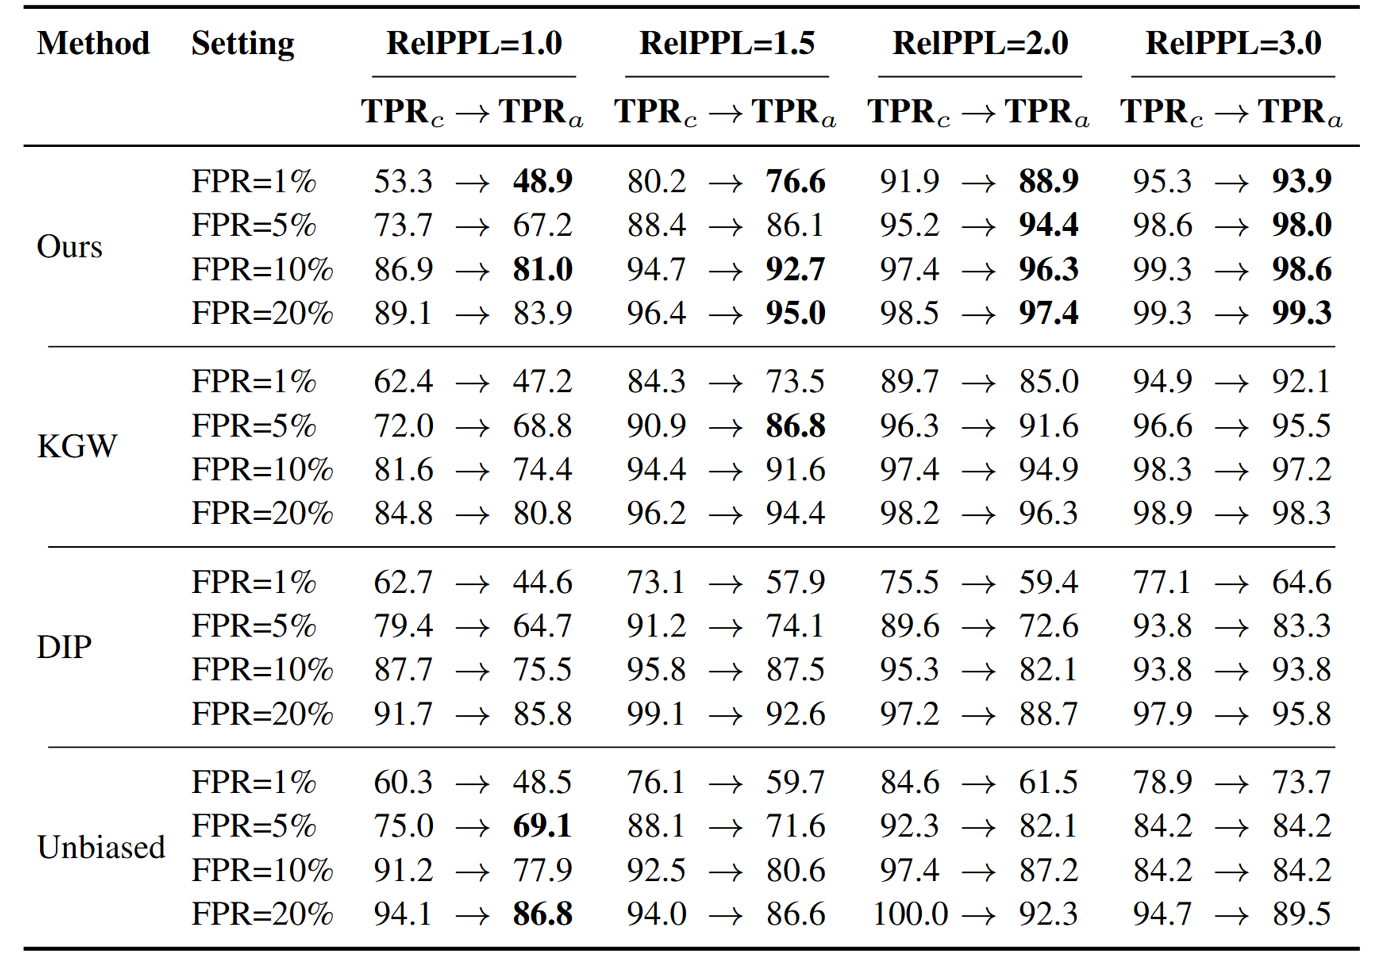
\includegraphics[width=\linewidth]{figures/tab_token_attack.png}
\end{table}

表~\ref{tab:token_attack_results} 给出了 token级扰动条件下的检测结果。表中每个单元格同时列出扰动前后的检出率，因此其中后一个数值直接反映了在固定编辑预算下仍可达到的检测水平。从整体结果看，在多数 RelPPL 分组与不同 FPR 设置下，本文方法的 $TPR_{\mathrm{attack}}$ 均保持在较高水平，并在较严格的误报率要求和较低 RelPPL 条件下表现出更稳定的检测能力。这表明，在轻度 token级改写存在时，本文方法仍能够较好地保留由水印引入的统计信号。

进一步地，与 KGW、DiP 和 Unbiased 等基线相比，本文方法在多数设置下的扰动后检出率更高，说明其鲁棒性优势并非仅体现在无扰动条件下的检测能力，而是体现在编辑后仍能够维持更高的可检测性。与此同时，可以观察到，RelPPL 较大的分组通常对应更高的扰动后检出率。这说明当带水印文本相对于无水印文本引入的偏移更明显时，其统计信号在相同编辑预算下也更容易被保留下来。

\begin{table}[H]
    \centering
    \caption{字符级扰动下的检测结果对比（Llama3-8B，编辑预算 $\varepsilon=0.01$）}
    \label{tab:char_attack_results}
    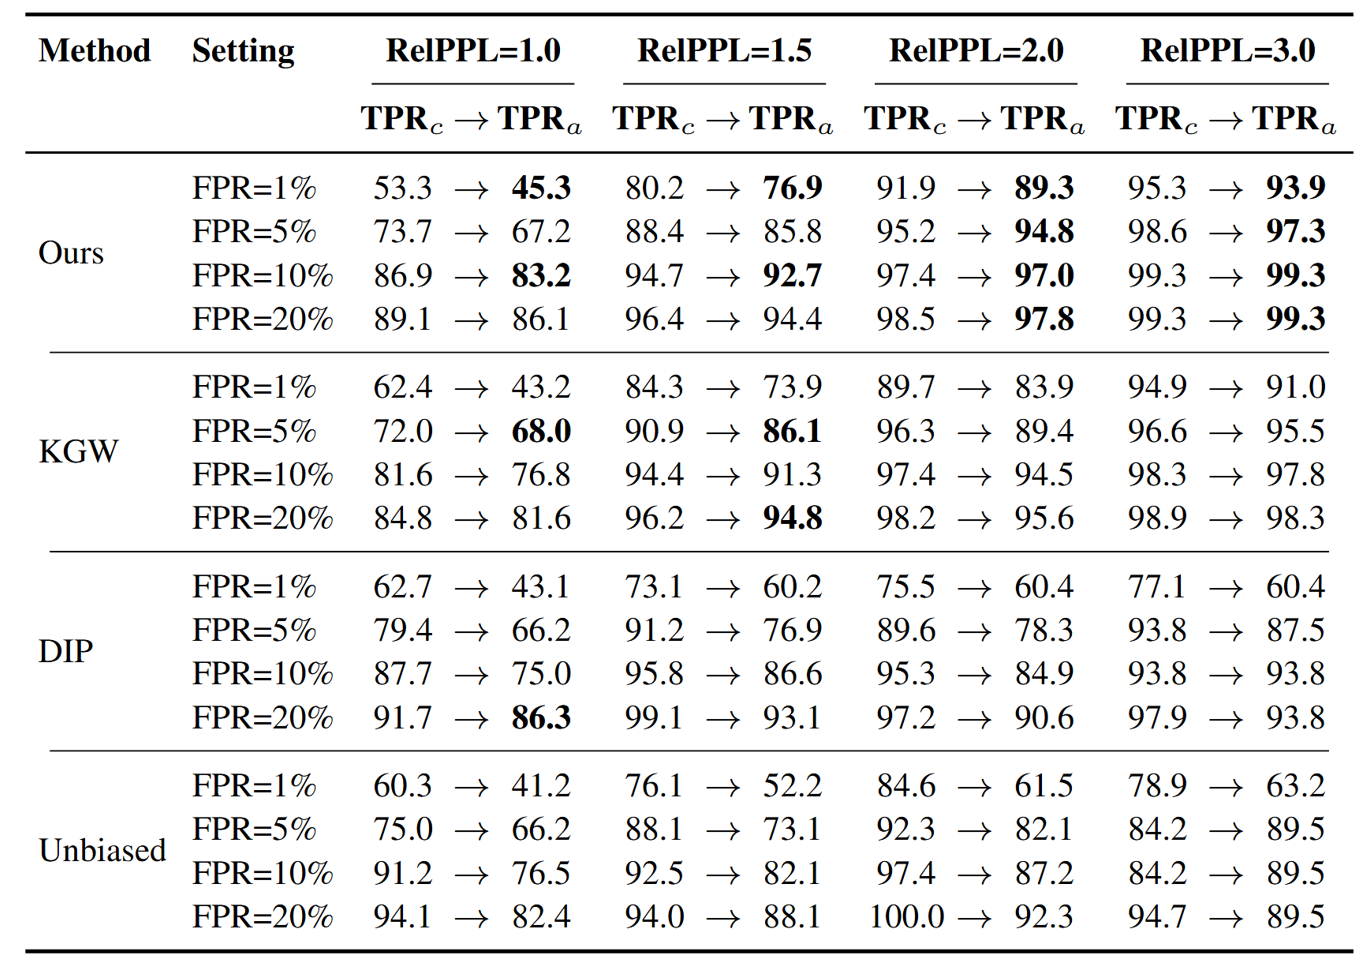
\includegraphics[width=\linewidth]{figures/tab_char_attack.png}
\end{table}

表~\ref{tab:char_attack_results} 给出了字符级扰动条件下的检测结果。相较于 token级扰动，字符级编辑更容易改变局部字节模式并进一步诱发分词边界变化。Zhang 等指出，这类微扰会通过分词级联效应放大检测退化\cite{zhang2025character}。Liang 等的综合评测也表明，此类攻击对依赖分词一致性的检测统计更具破坏性\cite{liang2024waterpark}。从表中结果可以看到，在多数 RelPPL 分组与不同 FPR 设置下，本文方法仍然保持了较高的 $TPR_{\mathrm{attack}}$，并在若干严格误报率条件下表现出较为稳定的检测能力。该现象说明，当前缀承载与指纹驱动分区同时作用时，字符级扰动虽然会削弱检测统计量，但并未彻底破坏检测端对绿色判定结构的重建能力。

对比表~\ref{tab:token_attack_results} 与表~\ref{tab:char_attack_results} 还可以发现，字符级扰动下的性能退化通常较 token级扰动更为明显。这与本章的问题设定是一致，因为字符级编辑更容易引发分词结果变化，因此对依赖绿色判定重建的检测流程构成更直接的挑战。Zhang 等从字符扰动引发分词级联效应的角度解释了这一现象\cite{zhang2025character}，Liang 等的综合评测也呈现出类似的退化趋势\cite{liang2024waterpark}。即便如此，本文方法在两类扰动条件下均保持了相对较高的扰动后检出率，说明其设计确实提高了对分词扰动的鲁棒性。

\begin{figure}[H]
    \centering
    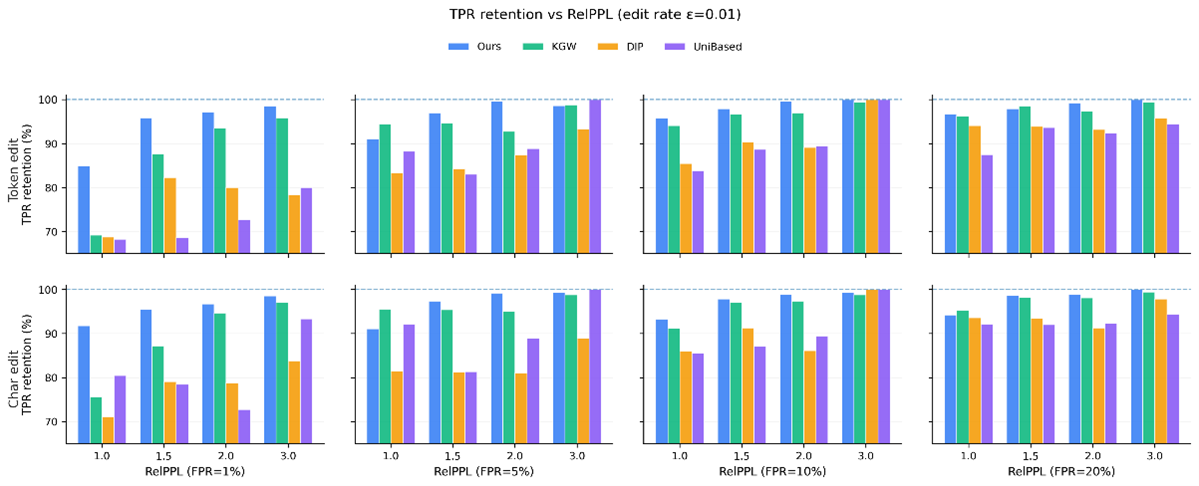
\includegraphics[width=0.92\linewidth]{figures/tpr_retention_relppl.png}
    \caption{固定编辑率（$\varepsilon=0.01$）下的检出率保持率}
    \label{fig:tpr_retention_relppl}
\end{figure}

除绝对检出率外，图~\ref{fig:tpr_retention_relppl} 进一步给出了固定轻度编辑预算下的检出率保持率，用于刻画扰动造成的相对性能下降幅度。图中分别展示了不同方法在 token级扰动与字符级扰动下的保持率，并按攻击前 RelPPL 进行分组。从结果可以看到，在多数分组与不同误报率设置下，本文方法的保持率更接近 $100\%$，或随分组变化呈现更平缓的下降趋势。这表明，在相同轻度扰动条件下，本文方法不仅在绝对扰动后检出率上占优，而且其检出能力的相对衰减幅度也更小。

总体来看，本节结果表明，在固定轻度编辑预算下，本文方法在 token级扰动与字符级扰动两种条件下均能维持较高的扰动后检出率，并在多数设置下优于对比方法。这说明前缀承载与指纹驱动分区的结合，能够在编辑扰动存在时更有效地保留可检测统计信号。下一节将进一步扫描更宽的编辑率范围，考察不同方法对编辑强度的敏感性。

\FloatBarrier
\subsection{编辑强度敏感性}

上一节在固定轻度编辑预算下，对不同方法的检测性能进行了比较。本节进一步扫描更宽的编辑强度范围，考察当编辑率 $\varepsilon$ 从 $0$ 增加到 $10\%$ 时，各方法检出能力的保留程度如何变化，从而刻画不同方法对编辑强度的敏感性。这里的编辑率 $\varepsilon$ 按扰动粒度分别计算：对于 token级扰动，以 token 数为分母；对于字符级扰动，以字符数为分母。

\begin{figure}[H]
    \centering
    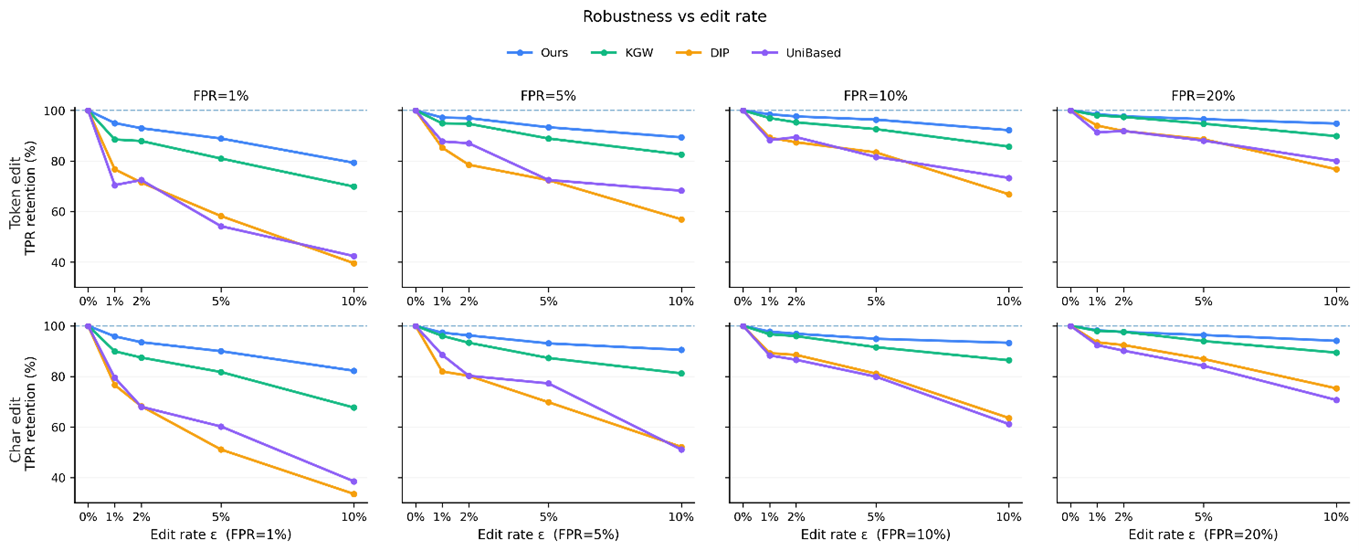
\includegraphics[width=0.90\linewidth,height=0.52\textheight,keepaspectratio]{figures/robustness_vs_edit_rate.png}
    \caption{不同编辑率下的检出率保持率}
    \label{fig:robustness_vs_edit_rate}
\end{figure}

图~\ref{fig:robustness_vs_edit_rate} 给出了不同编辑率条件下各方法的检出率保持率曲线。图中横轴为编辑率 $\varepsilon$，纵轴为检出率保持率 $\mathrm{Retention}$，其定义见式~\eqref{eq:retention}。上排对应 token级扰动，下排对应字符级扰动；每一列分别对应不同的误报率设置。曲线的整体高度反映了在给定编辑强度下仍能保留多少原始检测能力，而曲线随 $\varepsilon$ 的下降速度则反映了方法对编辑预算的敏感性。

从总体趋势来看，随着编辑率 $\varepsilon$ 增大，各方法的保持率普遍下降，说明编辑扰动会持续削弱文本中的水印统计信号。然而，不同方法的下降速度存在明显差异，这表明它们对编辑扰动的敏感性并不相同。总体而言，本文方法在多数编辑率档位和不同误报率设置下都保持了更高的曲线位置，并表现出相对更平缓的退化趋势，说明其对编辑强度的敏感性更低。

在 token级扰动条件下，本文方法在多个误报率要求与多个编辑率档位中均保持了较高的检出率保持率。特别是在编辑率进入较高区间（如 $5\%$ 至 $10\%$）之后，各方法的性能都出现进一步下降，但本文方法的退化幅度相对较小，仍能够维持较好的检测保留水平。这说明在以 token 为单位进行替换或改写时，本文方法引入的统计信号更不容易被快速破坏。

在字符级扰动条件下，保持率在多数设置下退化更为明显。这表明，字符级编辑比 token级编辑更容易改变局部字节模式并进一步诱发分词边界变化，从而对检测端重建绿色集合造成更强干扰。Zhang 等指出，字符级微扰会通过分词级联效应放大这种退化\cite{zhang2025character}。Liang 等的综合评测也表明，字符扰动下的检测保持通常更难维持\cite{liang2024waterpark}。即便如此，本文方法在多数误报率要求下仍表现出相对更高的保持率，或者呈现出更平缓的下降趋势。这说明当前缀承载与指纹驱动分区共同作用时，方法在分词扰动更显著的条件下仍能够较稳定地保留可检测信号。

从不同误报率设置的对比还可以观察到，当判决标准由严格逐步放宽时，各方法的保持率曲线整体上移，但不同方法之间的相对差异在多种误报率要求下都仍然存在。换言之，本文方法的鲁棒性优势并不依赖于某一个特定的误报率设定，而是在不同严格程度的误报控制条件下都表现得较为稳定。

进一步地，为解释图~\ref{fig:robustness_vs_edit_rate} 中检出率保持率随编辑率升高而下降的原因，本文统计了若干与可复现性相关的辅助量，并将结果汇总于表~\ref{tab:robustness_stats}。这些统计量并非主检测指标，而是用于从承载一致性、绿色判定稳定性以及分词结构变化三个方面，对鲁棒性退化的来源进行分析。需要说明的是，表中的 UID match rate 对应本文所说的前缀类别一致率，即扰动前后同一可对齐位置的承载类别保持一致的比例。

\begin{table}[H]
    \centering
    \caption{不同编辑率下的鲁棒性辅助统计量}
    \label{tab:robustness_stats}
    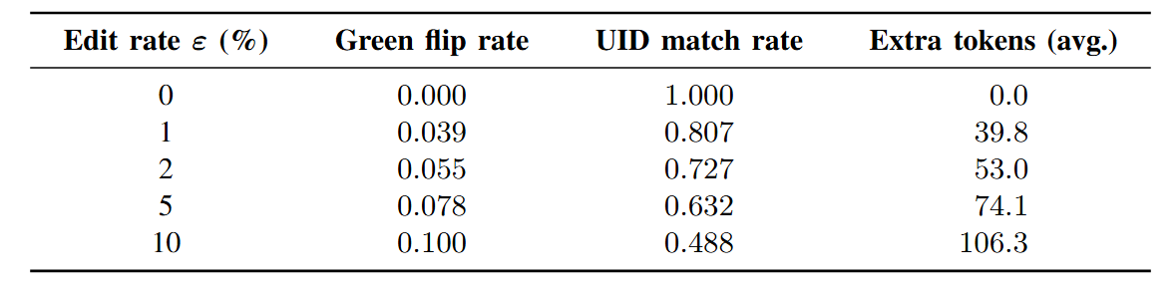
\includegraphics[width=0.88\linewidth]{figures/tab_robustness_stats.png}
\end{table}

表~\ref{tab:robustness_stats} 中包含三项辅助统计量。第一项为绿色判定翻转率，用于刻画扰动前后同一可对齐位置的绿色判定是否保持一致；该值越大，说明分区判定对扰动越敏感。第二项为前缀类别一致率，用于反映扰动前后承载类别保持一致的比例；该值越大，说明承载层在分词扰动下越稳定。第三项为平均额外 token 数，用于刻画扰动后相对于原文本新增的 token 数均值；该值越大，通常意味着分词边界漂移与长度膨胀越明显，从而使检测端在逐步重建绿色集合时更容易出现偏差。

从整体趋势看，随着编辑率 $\varepsilon$ 从 $0$ 增大到 $10\%$，绿色判定翻转率持续上升，前缀类别一致率持续下降，平均额外 token 数则明显增加。这表明随着扰动增强，局部分词结构和绿色判定的一致性都在不断退化，检测端越来越难以复现生成阶段所累积的统计结构。这一趋势与图~\ref{fig:robustness_vs_edit_rate} 中保持率随编辑率升高而下降的现象是一致的。

上述退化主要来自字符级编辑对文本表面形式与分词结果的共同影响。一方面，字符插入、删除或替换会改变局部字节模式，使分词器更容易产生边界变化，从而导致平均额外 token 数随编辑率升高而增加；另一方面，局部窗口内容的变化又会进一步影响上下文指纹的计算，进而引起部分位置绿色判定翻转，使绿色判定翻转率上升。Zhang 等指出，字符级微扰会通过分词级联效应进一步放大这一过程\cite{zhang2025character}。Liang 等的综合评测则表明，分词边界漂移与局部内容变化叠加后，更容易导致依赖分词一致性的检测结构失稳\cite{liang2024waterpark}。同时，分词边界漂移和局部内容变化叠加后，也会降低扰动前后承载类别保持一致的比例，从而表现为前缀类别一致率下降。

尽管扰动增强会导致上述统计量整体退化，但表~\ref{tab:robustness_stats} 也表明，本文方法在中高编辑率下仍保留了一定程度的承载一致性与判定稳定性。例如，在较高编辑率条件下，前缀类别一致率虽明显下降，但仍未退化到完全失配；与此同时，绿色判定翻转率虽然上升，但整体量级仍处于有限范围内。这说明本文提出的前缀承载与指纹驱动分区设计，在实际扰动条件下仍能够保留部分可复现结构，从而为检测端维持统计显著性提供基础。

综合来看，本节结果表明，编辑率增大会持续削弱各方法的检测能力，但本文方法在 token级扰动与字符级扰动两种条件下，对编辑强度的敏感性相对更低，表现为更高的检出率保持率或更缓的退化趋势。进一步结合表~\ref{tab:robustness_stats} 中的辅助统计量可以看出，这种鲁棒性优势来自两个层面的共同作用：其一，前缀承载降低了承载对象对精确分词边界的敏感性；其二，指纹驱动的分区机制在轻量扰动下仍能较大概率维持绿色判定结构的一致性。因此，本文方法能够在一定编辑预算范围内更有效地保留可检测统计信号。

\section{本章小结}

本章围绕字符级与 token级编辑引发的分词扰动问题，提出了基于前缀承载的水印算法。针对传统推理期文本水印对具体 token 身份与精确分词边界依赖较强、在编辑后检测结构容易失稳的问题，本文将水印承载对象由完整 token 身份提升为更稳定的前缀类别，并进一步引入由局部上下文指纹驱动的伪随机分区机制，从而减弱水印判定对精确分词边界和分词单元身份的依赖。在此基础上，本文构造了相应的偏置注入与统计检测流程，使水印信号能够在分词扰动条件下更稳定地保留下来。

实验结果表明，在不同误报率要求下，本文方法在 token级扰动与字符级扰动条件下均能够保持较高的扰动后检出率，并且随着编辑率增大，其检出率保持率退化相对更缓。进一步结合绿色判定翻转率、前缀类别一致率以及平均额外 token 数等辅助统计量可以看到，编辑率升高会导致分词漂移加剧、承载一致性下降以及绿色判定翻转增多，从而共同推动检测性能下降；与此同时，本文方法在一定扰动范围内仍能够维持较好的承载稳定性与分区一致性，说明所提出的前缀承载与指纹驱动分区设计在分词扰动场景下能够发挥作用。总体来看，本文方法在编辑后文本中更有效地保留了可检测统计信号，为提高推理期文本水印在真实传播环境中的鲁棒性提供了一种可行方案。






